\documentclass[a4paper,12pt,oneside,openright,final]{memoir} %twocolumn,

\let\footruleskip\undefined
\usepackage[utf8]{inputenc}
\usepackage[russian, ukrainian, english]{babel}
\usepackage{etex}
\usepackage{times}
\DisemulatePackage{setspace}
\usepackage{setspace}
\usepackage{amssymb}
\usepackage{amsfonts}

\usepackage{graphicx}
\usepackage[printwatermark]{xwatermark}
\newwatermark[allpages,color=red!10,angle=45,scale=5,xpos=-15,ypos=30]{DRAFT}

\usepackage{alltt}
\usepackage{moreverb}
%for more info on hyperref package see http://en.wikibooks.org/wiki/LaTeX/Packages/Hyperref
\usepackage[pdftex,colorlinks=true,linkcolor=blue, citecolor=magenta]{hyperref}
\usepackage{eso-pic}
\usepackage{transparent}
\setlength{\columnsep}{3em}

\usepackage{tcolorbox}
\usepackage{listings}
\definecolor{codebgcolor}{HTML}{6E84D6}  
\definecolor{codefgcolor}{HTML}{000000}% 071D70
\definecolor{basiccolor}{HTML}{000000}%1435AD
\definecolor{stringcolor}{HTML}{050505}% 2C3E82
\definecolor{highlight}{HTML}{FFB100}
\definecolor{annotationbgcolor}{HTML}{FFD473}

\usepackage{wrapfig}
\usepackage{caption}
\usepackage{subcaption}
\usepackage{alltt}
\usepackage{moreverb}
% tikz related packages to provide scalable graphics 
\usepackage{tikz}
\usetikzlibrary{calc,mindmap,backgrounds,positioning,arrows,shapes,shapes.arrows,shapes.misc,automata,petri,patterns,scopes,chains,matrix,decorations.pathmorphing,shadows,calc}

\usepackage{geometry}
\geometry{hmargin={15mm,15mm},vmargin={15mm,20mm}}

\usepackage[pages=some]{background}

\backgroundsetup{
  scale=1.2,
  angle=0,
  opacity=0.4,
  contents={
    
\includegraphics[width=1.1\paperwidth,height=1.1\paperheight, keepaspectratio]{images/00-background.png}} 
}


%%%%%%%%%%%%% copyright %%%%%%%%%%%%%%
\title{Trident Genesis Platform}
\author{Fielden Management Services Pty. Ltd.}
\date{}
\usepackage{hyperxmp}
\hypersetup{
    pdftitle={Trident Genesis Platform},
    pdfauthor={Fielden Management Services Pty. Ltd.},
    pdfsubject={A hight level overview of key principles and advantages.},
    pdfcopyright={Copyright (C) 2016 by Fielden Management Services Pty. Ltd.  All rights reserved.}
}

\usepackage{xcolor}
\makeevenhead{headings}%
    {\thepage}{}{\slshape\bookname~\thebook\qquad\partname~\thepart\qquad\leftmark}
    \makeoddfoot{headings}{\slshape\rightmark}{\color{gray}Copyright (C) 2016 by Fielden Management Services Pty. Ltd.  All rights reserved.}{\thepage}
	\makeoddhead{headings}{\slshape\rightmark}{}{}


\copypagestyle{headingsnobook}{headings}
\makeevenhead{headingsnobook}{\thepage}{}{\slshape\leftmark}


\begin{document}
\maketitle
\counterwithout{figure}{chapter}

\lstset{language=Java,
	  escapechar=\%,
	  numbers=left, numberstyle=\tiny, basicstyle=\tiny, basicstyle=\scriptsize\color{basiccolor}, stepnumber=1, numbersep=5pt, keywordstyle=\bfseries\color{codefgcolor}, stringstyle=\color{stringcolor}}

\onehalfspacing

%\BgThispage

\section*{Background}

	A significant number of enterprise software systems fail while still in development or fail to deliver on their promise from the business perspective\footnote{Some resources indicate up to 68\%.}.  
  	Recognising the fact that this problem has multiple causes (e.g. organisational, requirement management, skills), we would like to specifically emphasise the aspect of \emph{software construction}, which we believe has a significant influence on both the initial system development as well as the change support of the deployed systems.  
  
  	Robert Martin, who is one of the strongest proponents of the importance of software construction, stated in his speech at the NDC~2012 conference that there were no significant improvements to the processes of software construction comparing to the results in object-oriented analysis of the 1990th. 
  	In his experience, today's prevalent software development practices, tools and frameworks result in obstructing the core purpose of software systems at the code level.
  	Numerous frameworks and libraries such as web and ORM frameworks on the one hand facilitate software development by simplifying low level technical aspects, but on the other hand completely shadow the actual model and purpose of software systems.  
  	
	In fact, in talking about a software architecture, the emphasis is often placed at the level of some technology stack rather than at the level of an information system in question.
	For example, in the not so distant past we could hear a lot about a ``client-server architecture'', ``LAMP architecture'' or ``Java EE architecture''.
	Nowadays, it is the ``microservices architecture'' that is at the centre of everyones' attention.
	Every decade or so brings a new ``solution'' in a form of a new technology stack, but constructing reliable enterprise software systems remains one of the most difficult problems in the software engineering.	
	This problem is important and there is a good understanding that approaching it by trying to fix the architecture at the level of a technology stack is insufficient.

    An influential work by Ivar~Jacobson~\cite{jacobson1992} describes an approach (aka OOSE) for designing software and implementing the core business functionality as a set of use cases that are independent from any specific technology such as a web framework or some communication protocol.
  	One of the intents of this approach is to enable easy migration of the core functionality (the business value) to any new or different software technology stack.
  	However, Jacobson's approach has two limitations that are important to our discussion:
	\begin{enumerate}
   		\item The part of the core functionality that provides a way to tap into the supporting technology (so-called boundaries) significantly complicates the development process.
   		\item The use case approach limits capabilities of the application by enforcing a rigid behaviour.
  	\end{enumerate}
  
	The first limitation forces developers to keep changing the implementation of boundaries whenever either the supporting technology or the core business functionality changes.
	The second limitation hides the domain model from the end-users by restricting interaction between the system and the end-users to the scope of predefined use cases.
	This corresponds to the \emph{conversational metaphor} as defined in~\cite{HHN1986}, which is natural for process-oriented software systems\footnote{The popularity of the process-oriented approach seems to be related to a widespread adoption of the imperative programming paradigm that heavily influences the overall design of software systems, including UI.}.

	Hiding the underlying business model complicates reasoning about a software system for both the users and the developers.
	This impedes communication between different stakeholders.  
	The \emph{world model metaphor}~\cite{HHN1986} emphasises the importance of a transparent representation of the business model at the User Interface (UI) level.
	This way users can directly interact with the model without any intermediate representations.
  	The application of the world model metaphor to the system design has been researched by Richard Pawson~\cite{pawson2001, pawson2004}.
  	His research resulted in creation of architectural pattern \emph{Naked Objects} and a framework of the same name.
  	The Naked Objects pattern reinforces the MVC pattern by promoting domain-oriented style for capturing the business model (M) and supporting an automatic generation of UI (VC) from that model.
  	By employing domain-orientated modelling, Naked Objects falls into the category of domain-driven design~\cite{haywood2009} that provides an alternative to Jacobson's approach for system design~\cite{evans2003, vernon2013}.
    
    This pattern has many shortcomings, but the core ideas behind it, such as \emph{world model metaphor} and the \emph{direct manipulation principle}, resonated with our understanding of how to approach the problem of designing and constructing reliable enterprise software.
        
    
\section*{Introduction}
    
	Trident Genesis (\texttt{TG}) is a software development technology for constructing highly maintainable information systems that model complex business domains\footnote{The complexity of a business domain is defined as the number and nature of interdependencies between different domain entities and properties within any individual entity.}.
	It has been created out of internal needs for our company to reduce the technical complexity, increase reliability and improve maintainability of our software, which represents a range of ERP/EAM systems.
	These include information systems for a variety of industries such as Air Traffic and Navigation Services, Rolling Stock, Chemical Industry, Fleet and Ambulance Services.
	There is an inherent complexity\footnote{As opposed to accidental.} in such systems due to the real world complexity of the equipment, assets and other physical or virtual artifacts that are used in those industries as well as complex interdependent business rules that govern them, such as safety and competency regulations, preventive maintenance cycles, inventory reordering, financial rules, plant shutdowns, temporal availability profiles etc.
	
	Effective communication between all stakeholders is a key in achieving the necessary goals in any undertaking.
	That is why we view any information system as a communication tool that should facilitate cooperation between all participants. 
	Property constructed system should facilitate cooperation between users, their cooperation with the developers of the system and the cooperation within the development team itself.
	In order to achieve this, a technology for constructing information systems should have an appropriate representation or abstraction that would support communication and a ubiquitous language~\cite{evans2003} that is shared by all stakeholders\footnote{This should be thought of as a well established terminology in a specific business domain.}.
	\texttt{TG} establishes such an abstraction in a form of an architectural pattern to model the business domain and to construct the User Interface that follows a \emph{direct manipulation} principle~\cite{shneiderman1982, shneiderman1983}.
	The latter represents the underlying domain model transparently, providing a way for users to directly interact with it.

	The developed architectural pattern is unique in approaching the design of information systems from the perspective of their three essential functions~\cite{oli2007}:
	\begin{enumerate}
    	\item \emph{Memory}: to maintain a representation of the state of a domain.
    	\item \emph{Informative}: to provide information about the state of a domain.
    	\item \emph{Active}: to perform actions that change the state of a domain. 
	\end{enumerate}  	
	In \texttt{TG} all these functions are modelled uniformly by consistently utilising the same programming primitives.
	This ensures structural consistency for all parts of the system, which makes it ideal for iterative development and later changes during the production lifecycle of a system.
		
	An information systems that is developed with \texttt{TG} is an object-oriented construct with a responsive HTML5 front-end, which supports desktop and mobile profiles, a relational database system for state persistence and an application server that is build on RESTful principles and can be easily scaled with technologies such as Docker and load balancing.
	
	We have developed \texttt{TG} for our own needs and successfully used it to provide our customers with better, more reliable software, which is used in mission critical operations.
	Our team of Delphi developers, who were accustomed to a very procedural, UI driven approach, was successfully trained to shift their thinking away from low level technical details and approach software development from a business domain modelling perspective, which is fostered by \texttt{TG}.
	Once foreign, the practice of domain-driven unit testing to validate the business model and rules became a part of normal day-to-day software construction routine.
	
	
	The following sections delve into more details about TG.
	This includes the discussion of the developed architectural pattern and the influence of the REST architectural style on the modelling at the level of objects; how is it used to ensure a uniform model of an information system and how does it satisfy the SOLID principles~\cite{SOLID}; why controlled mutation it important and how immutability helps prevent accidental mistakes; how unit testing becomes domain-driven and why business processes could benefit from becoming persistent.
	We also discuss the Entity Query Language (EQL) for simple and non-trivial data querying and how the direct manipulation principle is employed for building consistent and intuitive user interfaces.
	This overview is concluded with a brief discussion of a fairly sophisticated information systems that is utilised in mission critical operations by one of our customers in the domain of Air Traffic and Navigation Services.


\section*{The architectural pattern of TG}
	The most common understanding of object-oriented programming is that ``it is useful for modelling the real world'', where there are objects with their behaviour.
	Taken literally, this perspective leads to many issues, including violation of SOLID principles that have, effectively, came to existence because of those issues.
	One such issue, which is important for the purpose of our discussion, is the lack of adequate means for representing verbs -- actions and processes\footnote{This issue is humorously  described by Steve Yegge in his ``Execution in the Kingdom of Nouns''~\cite{yegge2006}.}.
	The essence of this issue is that verbs do not exists in their own right and must be a part of some object (noun), represented as its behaviour in a form of a method\footnote{This is why it is so easy to violate the single responsibility or the open/closed principles.}.
	The same issue got translated into and plagued some of the distributed computational models such as Remote Method Invocation (RMI) and Simple Object Access Protocol (SOAP).
	The same issue makes it difficult to reason about objects' behaviour (too many methods, what is the state of the object they are invoked on, etc) and the same issue obstructs building \emph{semantically transparent}\footnote{The term \emph{semantically transparent} means a system where its underlying model is exposed for a direct manipulation by users.} information systems.
	
	The Naked Objects pattern attempts to follow the idea of the direct manipulation principle to transparently represent objects in UI.
	Naturally, it exposes the state as object properties for users to change them directly via UI, but in order to provide the behaviour, it exposes some of the methods as UI actuators (e.g. buttons, menu items) that can be invoked on an individual object.
	The approach of exposing object methods, introduces new issues and opens up many questions.
	For example:
  	\begin{itemize}
    	\item There is a need to differentiate between methods (i.e. behaviour) that can and cannot be exposed via UI;
		\item Why are there methods that are not exposed to UI -- doesn't this go against the idea of semantic transparency?
		\item If the exposed methods have arguments then how should their values be provided when invoking them from UI?
		\item What to do if some computation needs to be applied to a subset of objects, not just a single one?
	\end{itemize}
	
	This suggests that the described problem of having no first-class support for verbs, significantly complicates, if not making it impossible, to construct semantically transparent information systems by following the currently most prevalent understanding of object orientation.

\subsection*{The REST of Object-Oriented Programming}	
	
	In our research we came across some original work by Alan Kay where he explains object-oriented programming from a very different perspective than the one currently in common use.
	This view is tersely summarised by Alan Kay in his clarification of the term ``object-oriented'' in~\cite{Kay2003}.
	According to Alan Kay, the complexity of behaviour in object-oriented systems should come from interconnectedness between objects rather than from their methods.
	He compared an object-oriented system with a system of networked computers, or computing nodes, that have simple and uniform communication interface for interaction.
	
	For us, this treatment of object-orientation resonated with the representational state transfer (REST) architectural style~\cite{Fielding2000}, where there is a well defined and uniform way for interacting with web resources.
	Typically, web resources in RESTful systems react to requests that are expressed only in terms of HTTP verbs such as GET, POST, PUT and DELETE.
	Therefore, if the complexity of the Internet could be uniformly expressed as a multitude of web resources that have only four or so verbs for interaction, wouldn't the same or similar constraint at the level of objects result in a functionally rich and uniform object-oriented system design?
	This is the hypothesis that underpins the approach to object orientation that is taken in TG.
	Essentially, the application of the REST style to an object-oriented design of an information system in terms of its \texttt{Memory}, \texttt{Informative} and \texttt{Active} functions, resulted in the development of an architectural pattern that became the foundation of TG.
	This pattern is titled \emph{Fractal Objects} as it explicitly articulates that complex system behaviour is achieved by combining structurally identical building blocks -- the fractal object.
	A \emph{fractal object} is a construct consisting of two objects -- an \emph{entity} and its \emph{companion}.
	It is the basic conceptual building block for both designing and constructing information systems based on TG.
	
	\paragraph{Entity Object.} 	
  	An \emph{entity object} models the structure of a business entity, including its associations with other entities.
	Unlike the anemic domain model~\cite{fowler2003}, an entity has the responsibility to ensure the correctness of its state.
	Any value that is being assigned to its properties is validated in accordance with a specified business rule.
	This includes a mechanism of inter property dependency with automatic revalidation of invalid dependent properties.
	
	\begin{tcolorbox}[title=Example: dependent properties]
	\footnotesize
		There could be two mutually dependent properties \texttt{dateFrom} and \texttt{dateTo} that represent a date period, which should not be inverted.
		If property \texttt{dateFrom} has value \texttt{'2016-03-01'} and an attempt is made to assign property \texttt{dateTo} to value \texttt{'2016-02-01'} then the latter would be marked as invalid without any actual change to its value (i.e. an entity cannot be mutated with invalid values).
		Value \texttt{'2016-02-01'} for property \texttt{dateTo} gets captured as \emph{an attempted value}.
		A subsequent attempt to change property \texttt{dateFrom} by setting its value to \texttt{'2016-01-01'} would be successful.
		Due to inter property dependency mechanism, successful assignment to property \texttt{dateFrom} automatically tries to repeat the previous attempt to assign value \texttt{'2016-02-01'} to invalid property \texttt{dateTo}.
		This time it is a success, because \texttt{'2016-01-01' < '2016-02-01'} -- property \texttt{dateTo} becomes valid and attains new value \texttt{'2016-02-01'}.
 	\end{tcolorbox}
	
	The validation rules are declared as part of property definitions in a form of a specifically designed annotation.
	Any particular property may have no, one or several validators declared.
	In case of several validators, their execution is sequenced in the order of declaration.
	The validation process stops at the first failed validator or if all validators succeed.
	A value gets assigned only if all validators succeed.
	The ability to declare multiple sequential validators fosters good separation between different validation rules and provides a convenient way for reusing the same validation rules in application to properties of the same type, even if they belong to different entities.
	Without going any further into details, it is important to emphasise that in real world systems, the validation process rarely operates only on the in-memory state and often requires an access to a database.
	The developed entity validation mechanism is specifically designed with this requirement in mind and does not follow an approach that is frequently used in simpler problem domains where property setters are used to place the validation logic.
	Instead, validators are represented by separate classes that are implement as a property \emph{before change} contract and are executed by the \texttt{TG} runtime before setter invocations.

	Attempts to assign invalid values do not raise any exceptions.
	Validation errors are treated as an entity meta-data and TG provides an API to work with that meta-data.
	The meta-data is not limited only to identifying erroneous entity properties and their causes, but also captures and maintains in-memory mutations such as the aforementioned attempted values.
	This information is very useful when implementing intricate business logic, including the validation logic, which may require the knowledge of the original\footnote{A property value becomes \emph{original} if it gets persisted into the database. It is used to differentiate between in-memory mutations and persistent state of an entity.} or previous property values.
	The same information is used by TG itself, for example, to automate UI creation and to facilitate user interaction with the system by automatically validating their input and reporting errors.	
	The example below illustrates how a property declaration can incorporate the knowledge about its validators, persistent nature and the dependent properties at the Java code level.
	
	\begin{tcolorbox}[sidebyside, righthand width=0.3\textwidth, title=Example: property declaration with multiple validators]
    \begin{lstlisting}[numbersep=2pt]
@IsProperty
@Persistent
@Dependent("locationSubsystem")
@BeforeChange({
   @Handler(WaTypeValidator.class),
   @Handler(ServiceLocationSubsystemValidator.class)})
private Service service;
    \end{lstlisting}
	
	\tcblower
		\tiny
		Property \texttt{service} of type \texttt{Service} in entity \texttt{WorkActivity} is declared as persistent, which means it gets saved into a database.
		Its values have to satisfy validators that are specified as part of \texttt{@BeforeChange} in that order.
		And it has a dependent property \texttt{locationSubsystem}, which needs to be revalidated if the value of this property gets changed.	
 	\end{tcolorbox}

	Figure~\ref{fig:wa} depicts a master view for entry and modification of \texttt{WorkActivity} entities.
	It represents a subset of \texttt{WorkActivity} properties that are needed for this specific view, which in this case includes property \texttt{service} from the example above.
	The UI subsystem in TG automatically derives representation for properties from the meta-data information that is provided by the entity definition and its state at runtime.
	This includes completely transparent reuse of the validation logic, handling of dependent properties etc.
	Therefore, interaction with an entity instance programmatically and via UI leads to the same result.
	
	\begin{figure}[!h]
  		\centering
        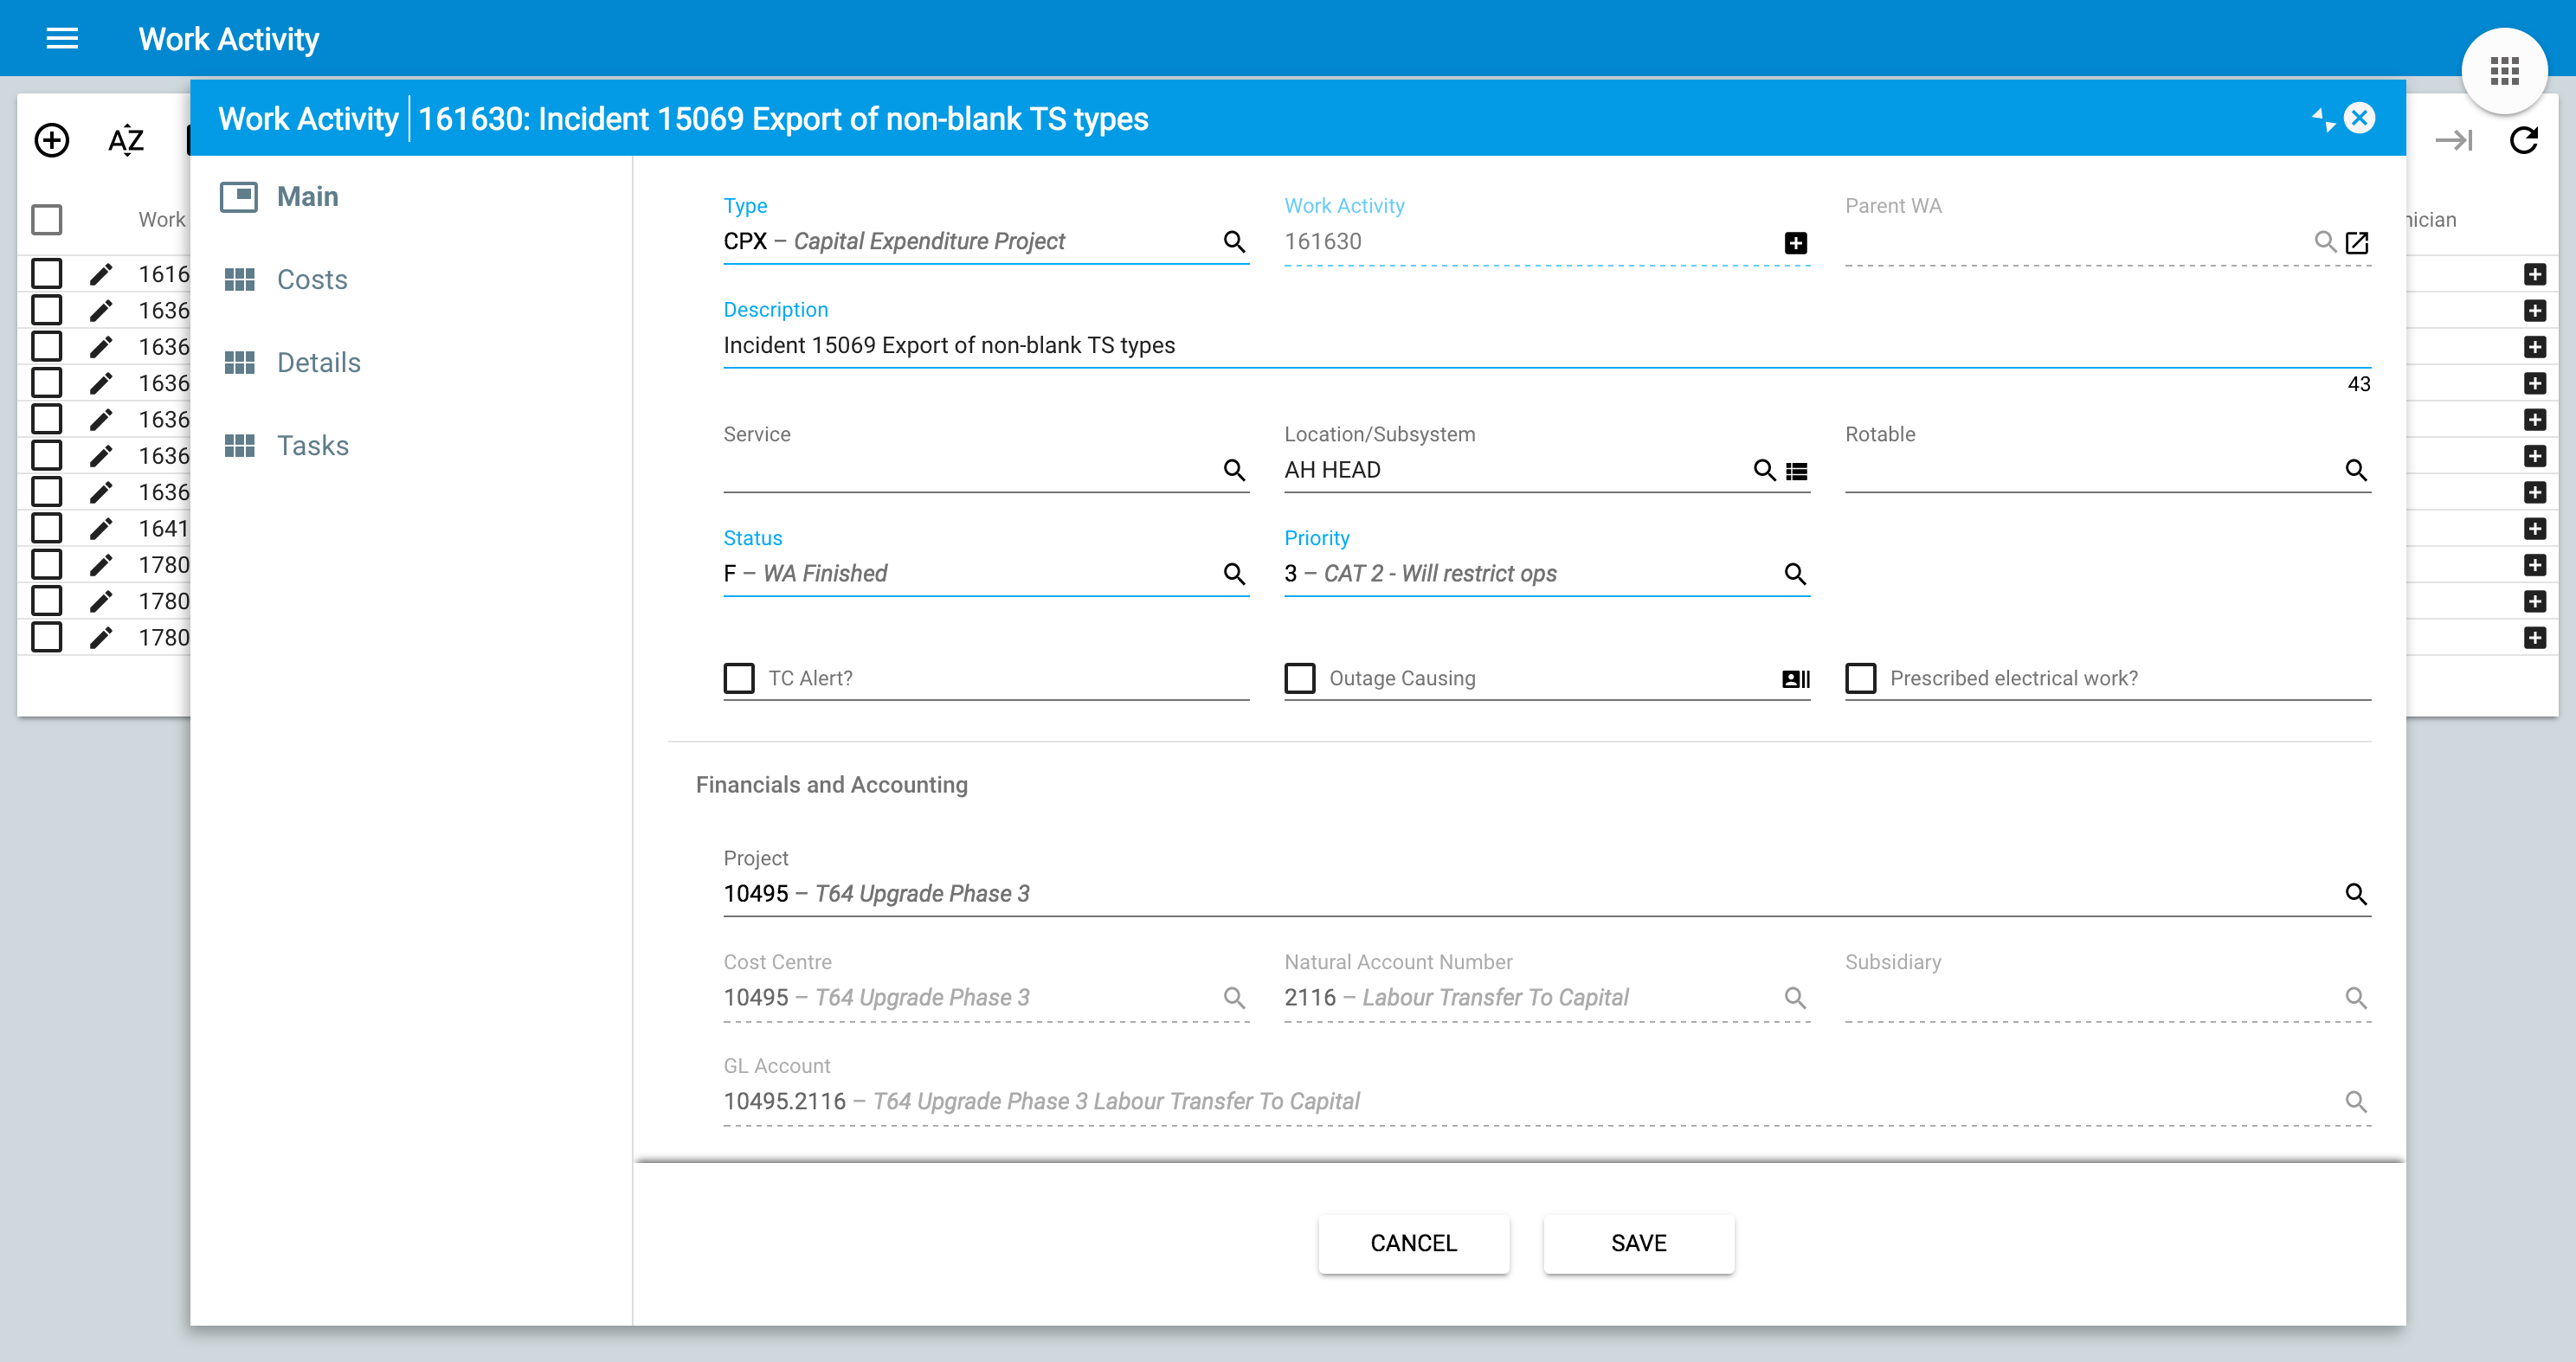
\includegraphics[width=1.0\textwidth]{images/01-wa-master.png}  
        \caption{Work Activity}
        \label{fig:wa}
		%\vspace{-30pt} 
  	\end{figure}

	One of the basic inherent property validations, is a check that properties that have an entity type, can only accept values that are already persisted.
	In our example, property \texttt{service} is of entity type \texttt{Service}.
	This entails that any value of this type must that is being set to \texttt{WorkActivity} property \texttt{service} must already exists in the application database.
	
	Figure~\ref{fig:non-existing-service} illustrates an attempt to assign a non-existing service \texttt{AA05IL}, which results in a validation error.
	There are several things that happen here.
	First, the user enters a textual value.
	Then, the system automatically recognises the intent by analysing the type of property \texttt{service} and tries to find an instance of type \texttt{Service} in the application database by using the entered textual value as a key search criteria.
	Having found no matching value, the system concludes that the basic validation failed, no subsequent validators are triggered and the error return to the client to be displayed to the user.

	\begin{figure}[!h]
  		\centering
     	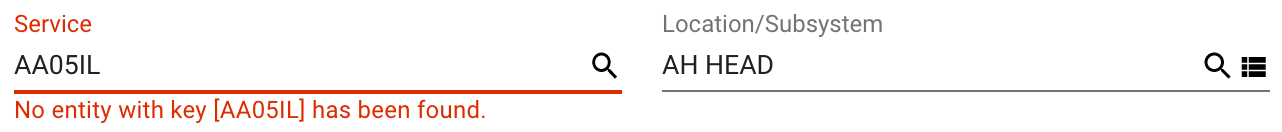
\includegraphics[width=1.0\textwidth]{images/02-wa-non-existing-service.png}  
  	  	\caption{Manifestation of validation in UI: invalid value.}
   		\label{fig:non-existing-service}
  	\end{figure}

	Figure~\ref{fig:dependent-validation} illustrates the situation where invalid value \texttt{AA05IL} is corrected by entering service \texttt{AA05ILS}.
	In this case, a single instance of type \texttt{Service} with key \texttt{AA05ILS} was successfully found in the database.
	That instance was passed to all subsequent property validators and eventually got assigned to property \texttt{service}.
	Due to this successful assignment and the declared dependency, property \texttt{locationSubsystem} in the same entity had to be revalidated as it could be have become invalid.
	However, the revalidation process did not fail~-- it resulted in a warning.
	This shows that the validation result does not have to be binary~-- success or failure -- there are many situation where value is acceptable, but users need to be informed of some consequential information.
	In this particular example, the user is informed that there are already open work activities for this location/subsystem.	
	
	\begin{figure}[!h]
  		\centering
      	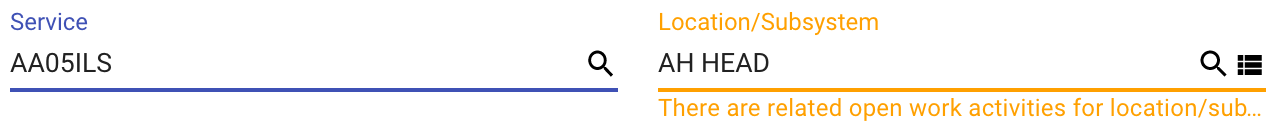
\includegraphics[width=1.0\textwidth]{images/03-wa-dependent-props.png}  
   	  	\caption{Manifestation of validation in UI: dependent property validation with warning.}
   		\label{fig:dependent-validation}
  	\end{figure}

	The example above is a very trivial and ubiquitous use case.
	It it important that all of the UI interaction gets automatically derived from the entity declaration without any ``intervention'' from the application developers.
	If a user reports a bug, for example, stating that some value should have been excepted, but wouldn't due to some validation error, the developers know exactly where to look for a potential error.
	It is very straightforward to setup a unit test that would try to reproduce the problem, and this is possible specifically because changing an entity state via UI and programmatically is equivalent.
	
	\vspace{8pt}
	In addition to property \emph{validators}, there is also support for, what we call, property \emph{definers}.
	Property definers get executed immediately after a successful property value assignment.
	This mechanism is very useful for complex business domains were a successful assignment of a property value should result in the assignment of the derived values to some other properties in the same entity or in a change to their meta-data such as their requiredness.
	Please consider the following example in application to an entry of \texttt{WorkActivity} where property \texttt{techinician} is assigned a new value.
	
	\begin{tcolorbox}[sidebyside, righthand width=0.38\textwidth, title=Example: property with a definer]
    \begin{lstlisting}[numbersep=2pt]
@IsProperty
@Persistent
@Required
@AfterChange(WorkActivityTechnicianDefiner.class)
private Technician technician;
    \end{lstlisting}
	
	\tcblower
		\tiny
		Property \texttt{technician} of type \texttt{Technician} in entity \texttt{WorkActivity} is declared as persistent and requried, which means it cannot be empty and gets saved into a database.
		There is only one intrinsic validator for checking value existence and does not require explicit declaration.
		This property has a definer, which is declared by using annotation \texttt{@AfterChange} and is executed upon each successful value change.
 	\end{tcolorbox}

	
	Figure~\ref{fig:tech} illustrates an entry of value \texttt{CRS} into property \texttt{technician}.
	This value is present in the application database as can be seen from the screenshot -- editors for properties of an entity type have the capability to autocomplete matching values\footnote{TG provides the default autocompletion logic, which can be enhanced at the application level, for example, to be context sensitive.}.
	
	\begin{figure}[!h]
  		\centering
      	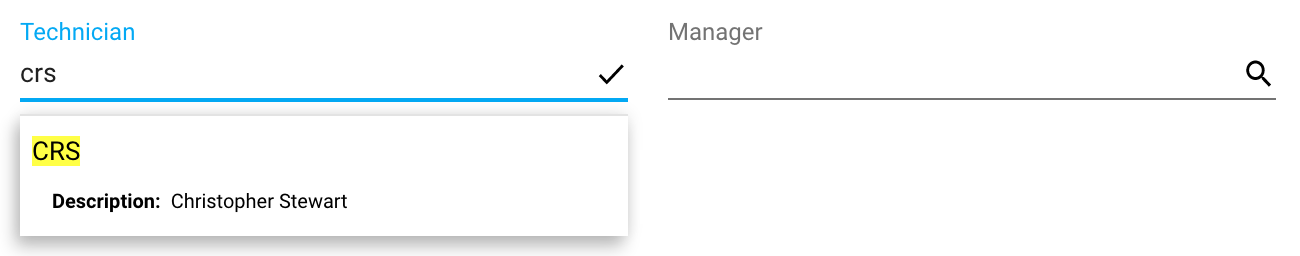
\includegraphics[width=1.0\textwidth]{images/04-wa-technician-entry.png}  
   	  	\caption{Selection of a value for property \texttt{technician}.}
   		\label{fig:tech}
  	\end{figure}
	
	Once the value is assigned, definer \texttt{WorkActivityTechnicianDefiner} is executed.
	This definer identifies if the entered technician has a manager.
	The manager of the entered technician gets assigned to property \texttt{manager} of the same work activity.
	Figure~\ref{fig:derived-manager} depicts the result of a successful assignment of value \texttt{CRS} to property \texttt{technician}, which resulted in an auto-assignment of a derived value \texttt{POM} to property \texttt{manager}.  

	\begin{figure}[!h]
  		\centering
      	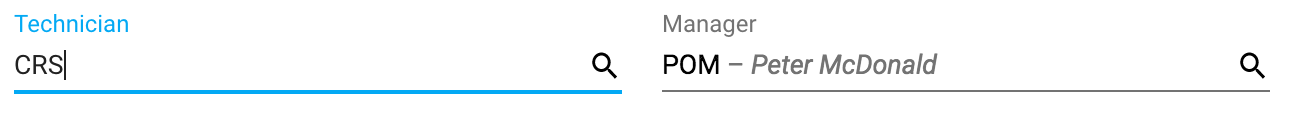
\includegraphics[width=1.0\textwidth]{images/05-wa-technician-entered.png}  
   	  	\caption{Auto-assignment of the derived value for property \texttt{manager}.}
   		\label{fig:derived-manager}
  	\end{figure}
	
	
	So far, we've discussed only the in-memory state modification and how the \emph{entity} part of a \emph{fractal object} is used to model and ensure correctness of a business entity.
	The examples above illustrate that in-memory changes require the ability to execute potentially complex validation rules, including communication with the application database.
	Changes to some properties may result in changes to some other properties.
	This shows that changing entity properties encompasses rich domain behaviour, which is captured at the entity model level declaratively and is transparently integrated with an application UI.
	The main \emph{takeaway} from this, is that the same business rules to verify an entity state validity are applied consistently regardless of where in the business logic or UI any particular entity instance is modified.
	This is a lot stronger guarantee than offered by other frequently used approaches where different ``services'' can change the same properties of the same entity, but with different and potentially inconsistent/contradicting validation business rules.
	
	\paragraph{Companion Object.}	
	A \emph{companion object} models the four basic operations that can be performed on a corresponding \emph{entity object}.
	It represents a RESTful interface to its counterpart entity object.
	Only by means of a companion object could an entity be \emph{created}, \emph{saved}, \emph{deleted}, and \emph{retrieved}\footnote{One could think of these operations as simple CRUD, but this analogy is misleading for reasons that will become evident further into the discussion.}.
	
	The power of having a limited number of operations has been demonstrated by the REST style~\cite{Fielding2000} of architecture for web applications.
	We argue that similar benefits are gained at the level of domain modelling.
  	There is a lot of semantic similarities between the REST style of web resources (macro level) and the objects modelling of a business domain (micro level).
  	For example, the use of URI paths to navigate between web resources is analogous to paths in object graphs for association traversal.
  	This resonates with the original view of object-oriented systems by Alan Key, who emphasised similarity between objects and networked computers.
  	Although, web is a delivery mechanism and a software system may or may not run on the web, its intrinsic nature of interconnected resources with uniform interaction mechanism seems to be very appropriate for an object-oriented modelling.

	The operations that are defined for companion objects are reminiscent of the \texttt{HTTP} verbs \texttt{PUT}, \texttt{POST}, \texttt{DELETE} and \texttt{GET}.
	As is the case with REST web resources, they may or may not be applicable to a specific entity object in question.
	For example, not all persistent entity objects that can be \texttt{saved} and \texttt{retrieved} from a database should necessarily support \texttt{deletion}.
	Another example could be of an entity that models a business process, such as purchase order authorisation.
	\texttt{Saving} such entity triggers the execution of a rich transactional business logic that affects multiple related entities, including changes to their persistent state.
	However, in itself, that entity could be transient and its properties serve only as parameters of the business process in question.
	
	As mentioned before, the conventional OOP thinking views a class as a basic building block or a module when applied to the modelling of a business domain.
	This leads to an ``understanding'' that an object should encapsulate and express its behaviour as methods of a class when modelling a business entity. 
	Thus, any object may have many, often unrelated, methods that try to capture different behavioural aspects of the same business entity.
	For example, with such approach entity purchase order could be modelled as class \texttt{PurchaseOrder} with separate methods to print purchase order, export purchase order, add purchase order line, authorise purchase order etc.
	This clearly violates at least the single responsibility principle~\cite{SOLID} and raises the question of adequate separation of concerns as class \texttt{PurchaseOrder} would need to be modified for multiple unrelated reasons such as changes in the export format requirements or the structure of a purchase order line object.
	In order to resolve these problems many software architectural styles introduce the notion of \emph{services} (e.g. domain services in Domain-Drive Design).
	Such approach does not solve the problem per se as it only represents an \emph{escape route} to move some ``unfitting'' (whatever the criteria for that is) behaviour from a class that represent a domain entity to another class, which is thought of as a ``service''.
	Also, this introduces an additional design concept that has the same set of problems -- what behaviour should it encapsulate, what methods should it expose etc.
	
	The use of a complementary pair of objects -- an entity and its companion -- as the basic system module, provides a well-defined contract to model an information system: entity objects are responsible for ensuring the correctness of their own state and there are only four clearly identified as part of their companion object operations to affect the overall state of an information system (e.g. save or delete data represented by entity objects).
	If an entity object represents a persistent domain entity then the only way for its instances to be persisted is by executing method \texttt{save} of a corresponding companion object -- the same business logic that is implemented as part of method \texttt{save} gets executed regardless of where in the system the method is invoked.
	Only valid entity instances can be saved and the only way to change an entity instance is by modifying its properties that enforce the validation rules.
	There is no way to bypass the validation logic when changing an entity and there is no other way than to use a correponding companion object to save new or modified entity instances.
	This achieves a uniform approach to the domain modelling where the business entities (e.g. purchase order), processes (e.g. purchase order authorisation) and complex data querying that may involve joining of multiple persistent entities (e.g. reporting the whole-life cost for an asset that encompasses repair, fuel and servicing cost components) is modelled with the same modelling primitives -- pairs of entity and companion objects.

	Such uniformity contributes significantly to the comprehension of an information system by both the original and new developers that just need to follow the established pattern to identify how different parts of the system interact with each other and what are the rules for that interaction.
	So, unlike in the case of more traditional approaches, there is no need to "think" what various behavioural methods that are defined as part of "domain objects" or "services" mean and what is their effect on the system.
	One only needs to "think" what does some entity object models -- the ways for it to effect the system are defined uniformly as four operations on a corresponding companion object.
	Combining this uniform approach with the direct manipulation principle for building UI, yields a very transparent system where users and developers can clearly identify problem areas that need bug fixes, improvement or enhancements.
	
	As an example, figure~\ref{fig:wa-detail} depicts an \emph{entity master} for a persistent entity \texttt{WorkActivityDetail} that models a domain entity for capturing details of some work being performed.
	There can be multiple entity instance of this type associated with the same work activity and any existing details can be edited under some conditions.
		
	\begin{figure}[!h]
  		\centering
        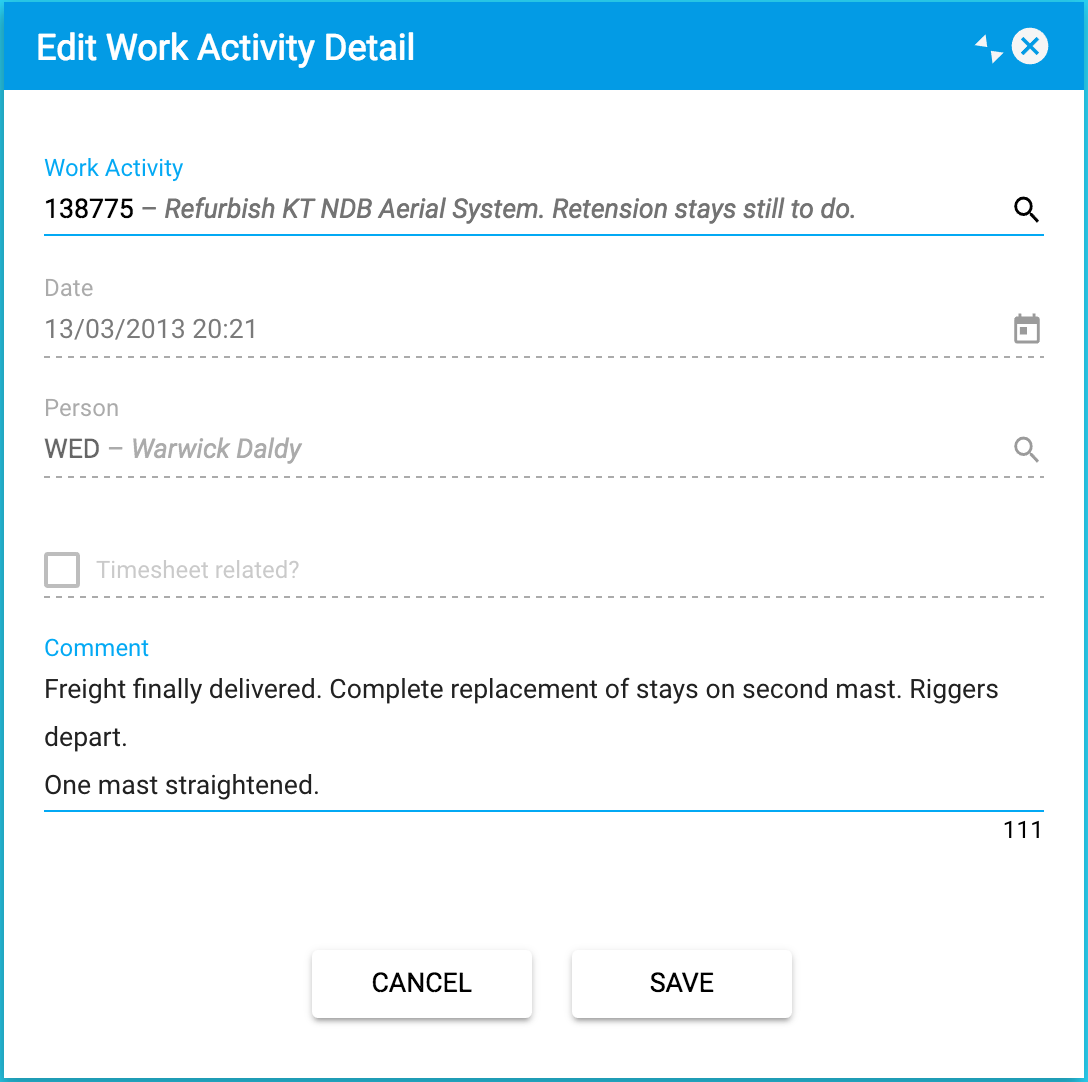
\includegraphics[width=.55\textwidth]{images/06-wa-detail-master.png}  
        \caption{Work Activity Detail}
        \label{fig:wa-detail}
		%\vspace{-30pt} 
  	\end{figure}

	Entity \texttt{WorkActivityDetail} has five properties.
	Three of those are read-only from UI perspective and can only be changed programmatically, the remaining two are required\footnote{This nature of properties is automatically taken into account in the UI layer by reusing the definitions that are captured at the domain model.}.
	Buttons \texttt{CANCEL} and \texttt{SAVE} are directly mapped to the two of four companion object operations -- \texttt{retrieve}\footnote{Cancelling changes is equivalent to refreshing an entity from a database by means of re-retrieving it.} and \texttt{save}.

	The code listing below illustrates a part of the implementation for companion object \texttt{IWork\-Activity\-Detail} of entity \texttt{WorkActivityDetail}.
	It extends a generic base class \texttt{CommonEntityCo} with a type parameter that is specified as the type of a corresponding entity object.
	This makes every concrete companion specialised to handle a single entity object.
	The base class is provided by the TG platform and encapsulates all the essential logic of saving persistent entities, which includes the construction of appropriate insert/update statements, optimistic locking mechanism, conflict resolution logic etc.

	Entity retrieval in this example is quite trivial and its only concern is to use an appropriate fetch model to obtain an object subgraph that would be sufficient for editing purposes.
	The \texttt{save} operation is represented by method of the same name and illustrates some of the important aspects that deserve a more detailed discussion.
	
	\medskip
	
	\begin{tcolorbox}[sidebyside, righthand width=0.3\textwidth, title=Example: simple \texttt{save} operation]
    \begin{lstlisting}[numbersep=2pt]
@EntityType(WorkActivityDetail.class)
public class WorkActivityDetailCo 
    extends CommonEntityCo<WorkActivityDetail> 
    implements IWorkActivityDetail {
    ...
    @Override
    @TransactionRequired
    public WorkActivityDetail save(
        final WorkActivityDetail detail) {
    
        if (detail.getTimesheet() == null && 
            detail.getProperty("comment").isDirty()) {
           detail
           .setDate(universalConstants().now())
           .setPerson(co(Person.class).currentPerson());
        }
    
        return super.save(detail);
    }
    ...
}    
	
	\end{lstlisting}
	\tcblower
		\tiny
		 Annotation \texttt{@TransactionRequired} represents a declarative transaction demarcation~-- all data changes in method \texttt{save} are wrapped into a single transaction.

		 \medskip
		 Method \texttt{save} expects a single argument, which is a new or modified entity instance of type \texttt{WorkActivityDetail}.

		 \medskip		 
		 The entity meta-data can be accessed via API to check what properties of the specified entity instance have been changed and what were their previous values.

		 \medskip		 
		 The business logic in method \texttt{save} can be very rich, affect other entities and depend on the changed properties.
		 
		 \medskip		 
		 A successfully saved entity is returned as the result of method \texttt{save}.
		 
 	\end{tcolorbox}	

	First of all, method \texttt{save} extends the inherited method \texttt{save}.
	The call to \texttt{super.save} is the only way to initiate the actual entity saving.
	This \texttt{super} call can appear anywhere in the body of the overridden method \texttt{save} as all the database changes in this method are atomic (belong to the same transaction).
	However, often such a decision is governed by the actual business logic that should be executed as part entity saving.
	In this case, it makes sense to call \texttt{super.save} as the last method instruction (line 18) in order to persist preceding entity changes -- lines 14 and 15.
	The returned instance represents a re-fetched entity.
	The re-fetching logic is based on an automatically reconstructed fetch model using an entity instance being saved (\texttt{detail} in this case).
	This guaranties that the returned instance contains the most fresh data in its object sub-graph.
	
	Method \texttt{save} expects a single argument -- a new or modified entity object that needs to be persisted.
	Lines 11--16 correspond to a business logic, which dictates that under certain condition properties \texttt{date} and \texttt{person} of \texttt{detail} (the entity being saved) should be updated with the current date/time and the currently logged-in person, who actions the change.
	The condition (lines 11 and 12) to update values for these properties checks if \texttt{detail} has a timesheet associated with it and if its property \texttt{comment} is dirty.
	The latter is an example of using meta-data API to identify if some property was changed, but not yet persisted.

	Entity properties are updated by invoking property setters (lines 13--15).
	Definitions of entity objects follow the idea of fluent API, which enables convenient chaining of setter calls.
	Property \texttt{date} is assigned the value, which is computed by expression \texttt{universalConstants().now()}\footnote{This expression encapsulates the notion of a \emph{model time} that provides a way to control time for testing purposes.}.
	Property \texttt{person} is assigned the \emph{current person} by obtaining an instance of a companion object for entity \texttt{Person} (i.e. \texttt{co(Person.class)}) and then calling its method \texttt{currentPerson()}.
	
	Method \texttt{IPerson.currentPerson()} is an example of operation \texttt{retrieve} that is expressed in more domain specific terms.
	The TG platform provides a necessary abstraction to identify the currently logged in application user.
	This abstraction has its implementations for testing and deployment purposes that get injected depending on the execution context.
	Entity \texttt{User} with its companion \texttt{IUser} are present at the platform level and can be accessed by the application specific domain logic.
	Entity \texttt{Person} is a domain entity, implemented at an application level.
	In the domain, which is used for this example, entity \texttt{Person} has many domain specific properties such as payment rates, normal and overtime hours, a supervisor etc.
	At the same time, each \texttt{Person} instance is in a unique one-to-one association with a corresponding instance of \texttt{User}.
	That is why it is possible and more natural to express the notion of a currently logged in user in terms of domain entity \texttt{Person}.
	
	The above example is very simple, but it should be sufficient to see that a companion operation \texttt{save} is capable of containing rich transactional business logic, which could affect a persistent state of an information system across multiple entity objects of different types.
	Having both entity properties and the operations of companion objects directly mapped to UI controls, guides the thought process when designing and using the system.
	It is always clear what changes need to be implemented at the code level whenever an application user refers to some functionality in terms of UI constructs.
	
	The next section delves more into the application of the Fractal Objects pattern to model the three essential information system functions (\texttt{Memory}, \texttt{Informative} and \texttt{Active}).
	It shows how approaching the design of an information system from the perspective of just these three functions by applying the FO pattern leads to a significant reduction of the architectural complexity.
	We also introduce Entity Query Language (EQL) as an essential part for communicating with an application database and constructing sophisticated queries that capture the information across multiple persistent (memory) entities to produce synthetic entities for reporting (informative) purposes.


\iffalse


	Surprisingly, I don't see in the other answers what i consider the real difference between REST and CRUD: what does each one manages.

	CRUD means the basic operations to be done in a data repository. You directly handle records or data objects; apart from these operations, the records are passive entities. Typically it's just database tables and records.

	REST, on the other hand, operates on resource representations, each one identified by an URL. These are typically not data objects, but complex objects abstractions.


	
	A service encapsulates entities and it protects consistency through the business logic. 
	If the original business request affects multiple entities, a service can only provide complete service if it gets enough information about the original request.
	Then it can execute the business logic, apply that business logic even across multiple entities, and maintain both information consistency and transactional consistency.
	
	%CRUD does not offer this.
	

	Unlike the rich domain model approach~\cite{evans2003},
	
	
	Design pattern \emph{Command} is a very good analogy for understanding \emph{Functional Entities}.
	The added value of using FO for modelling functional entities has to do with the behaviour that is provided by an entity object such as property validation, dependency handling etc.


	Unlike the anemic domain model~\cite{fowler2003}, an entity has the responsibility to ensure the correctness of its state.
	
	
		
	
 
\subsection*{Computing Platform}

	In theory of data modelling, a conceptual data model is defined as a pair of languages~-- a data definition language and a data manipulation language~\cite{kal1983}.
  	This definition was effectively used in relational data modelling whereby both languages have been implemented as Structured Query Language that supports data definition and manipulation.
  	Having a data model described in terms of SQL allows one to easily move this model and associated data instances between different RDBMS system with very little if any changes.
  	At the same time concrete RDBMS implementations are very specific, have their own algorithms and optimisations techniques to effectively manage the data described by such generic models.
  	This demonstrates the power of the conceptual data model that is desirable for any information system.
  
  Our research hypothesis is that a similar conceptual model can be effectively applied for modelling information systems using general-purpose object-oriented languages.
  Such model should have a language to describe a business domain (both structural and functional aspects) and a language for manipulation of the artefacts that are resulted from such description.
  There should also be a computing platform that could run any concrete domain model similarly to an RDBMS system that can run any concrete data model described with SQL.
  
  One could compare this to a generative or automatic programming approach, but there is a very clear distinction -- generative programming relies on code generation that in many cases requires to be modified manually in order to achieve the required behaviour.
  This manual modification often leads to breaking of the original model that was used for code generation.
  That is why the analogy with SQL is better -- SQL code gets interpreted, and even some optimised code could be generated from it, but never do we change any SQL code representation that is actually executed by RDBMS.
    
  The main purpose of a computing platform is to abstract out the technologies required to run the resulting software system.
  For the purpose of our research we had very specific requirements to the computing platform that would ensure the robustness of our hypothesis testing.
  The most important of them are:
  \begin{itemize}
    \item The dependency between the platform and the model should only exist in the sense that the platform ``understands'' both the definition and manipulation languages used for modelling a business domain.
    \item The platform should segregate the details of persistence and communication mechanism allowing it to be executed on a single machine, across the LAN or the Internet.
    \item The platform should provide an automatic generation of UI from the model that would follow the direct manipulation human-computer interaction style~\cite{shneiderman1982, shneiderman1983}.
  \end{itemize}

  The first requirement indicated the need for loose coupling between domain models and the actual computing platform that can execute them.
  It should ensure that changes in the internal (not the interfacing) parts of the computing platform would not require to change the domain model.
  The goal of the second requirement is to take away low technical details away from software system developers, so that they could concentrate on the immediate business value -- modelling of the domain.
  The last item emphasises the fact that the computing platform should specifically address the way users interact with the system in order to facilitate semantic transparency from user experience perspective.

  Therefore, the means to describes the domain model and the computing platform that can execute such models are the two essential parts of Fractal Objects.
  The developed prototype of the Fractal Object approach has been done in the Java programming language, but any other object-oriented language could be used.
  Java is still one of the most widely used programming languages and proved to be well suited for the implementation of transactional business systems.
  However, our decision to use Java was also influenced by its rich reflection capabilities that allow runtime introspection in order to gather metadata, and its use of interfaces to support polymorphism that could be effectively used by the platform for inversion of control to enable loose coupling with domain models.





\section*{The problem statement}

	It puts the modelling of a business domain in the centre of software requirement management, design and construction by following a very specific architectural pattern called \emph{Fractal Objects}.
	The unique trait of the \emph{Fractal Objects} pattern is in establishing a uniform approach for designing and implementing the three core functions of any information system~-- memory, informative, active~\cite{oli2007}.
	This results in a holistic system design and implementation that is maintainable and of high fidelity with the target business domain.

	The current definition and functions of an information system was defined back in 1970s.
	

	
	There are two metaphors in the context of information systems construction -- conversational and world model.
	They convey the meaning of two very different principles that underpin an information system -- both with their cons and pros.
	
	More traditional, but now again in the centre of everyones' attention due to the raise of micro services, is the conversational metaphor.
	Information systems that follow it, do not permit a direct interaction of users with an underlying data model.
	Instead, a UI and API layers act as an intermediary, hiding the underlying model of an information system.
	
	The world model metaphor emphasises the direct manipulation principle where users query and change the data by interacting with the underlying model.
	
	Any data model can be viewed as a pair of languages -- a language for describing the data and a language for interacting with it.
	For example, in relational databases, the Data Definition Language (DDL) is used to describe the data and the Structured Query Language (SQL) is used to interact with it.
	A data model is central to any information system.
	Thus, the pair of languages is for defining and interacting with the data is of the essence.



\section*{What is Trident Genesis?}
  Trident Genesis (TG) is an opinionated software platform for developing business applications in a domain driven way.
  It lifts the level of abstraction up to the modelling of the business domain, while automatically handling low level technical details.
  
  \vspace{3 mm}
  \noindent The architecture of the business domain is often unique. 
  This is what makes companies competitive.
  Capturing the business domain model in a form of a functional software system that facilitates business operations represents the core value for customers.
  
  \vspace{3 mm}
  \noindent The TG platform incorporates over 30 years of experience in delivering Enterprise grade software solutions at a software architecture level.
  It encapsulates the complexity of the low technical details for efficient database communication, concurrent data processing, HTML5 client construction enabling software developers to concentrate on the business domain architecture.

\begin{figure}[!h]
    \vspace{-5pt} 
    \centering    
    \begin{tikzpicture}[node distance=1cm, auto, opacity=0.8, scale=0.7, every node/.style={scale=0.7}]
      \tikzset{
	  mynode/.style={rectangle,rounded corners,draw=black, top color=white, bottom color=blue!50,very thick, inner sep=1em, minimum size=3em, text centered, text=blue!50!black},
	  platform/.style={rectangle,rounded corners,draw=black, top color=white, bottom color=green!50!white,very thick, inner sep=1em, minimum size=3em, text centered, text=green!50!black}
      }  
      \node at (1, 1) [mynode] (ap1) {Application};
      \node at (1.7, 1.7) [mynode] (ap1) {Application};
      \node at (2.4, 2.4) [mynode] (ap1) {Application};

      \def\platformpath{-- +(5cm,0cm) -- +(5cm,2cm) -- +(3cm,2cm) -- +(3cm,2.5cm) -- +(4cm,2.5cm) -- +(2.5cm,3.5cm) -- +(1cm,2.5cm) -- +(2cm,2.5cm) -- +(2cm,2cm) -- +(0cm,2cm) -- cycle}
      \draw (-1,-3.3) [platform] \platformpath 
	    node [below,text width=7em, text centered,xshift=2.2cm,yshift=0.8cm] {Trident Genesis Platform};  
    \end{tikzpicture}
    \vspace{0pt} 
  \end{figure}

  \noindent The typical software construction workflow with TG encompasses: modelling of the business domain (declarative ontological aspect), implementing core business rules (imperative aspect) and configuring the user interface.
  These steps are facilitated by high level abstractions provided by the platform.
  The platform enables developers to concentrate on the modelling of the business domain. 
  This ensures higher productivity, quality and value of the final software system for the business.


 \subsection*{Principles and Advantages}
  	TG is designed to ensure that the application facilitates communication between different business stakeholders and is easy to use by incorporating the following principles and approaches.

\subsection*{Unique object-oriented architectural style to uniform modelling of the business domain}
	One could argue that commanding a programming language is relatively easy. 
  	However, object-oriented design is a different story.
  	It takes many years to become an experienced software architect.
  	TG provides a well defined architectural style that not only solves low technical tasks, but most importantly incorporates a unique architectural approach to uniform modelling of the business domain.
  	The platform ensures that all TG-based applications follow exactly the same development and modelling style, which leads to structural and behavioural uniformity of the final software system.
  	This protects developers from a multitude of programming errors.
	It enables agile development of working solutions that can be easily supported by both the original or new developers.

    \begin{figure}[!h]
    %\vspace{20pt}
    \centering    
    \begin{tikzpicture}[>=latex', scale=1.0, every node/.style={scale=1.0}]
      \tikzset{
	  outercore/.style={circle, fill=blue!50!white, inner sep=0em, minimum size=0.6cm},
	  core/.style={circle, shade, ball color=green!50!white, inner sep=0em, minimum size=0.3cm},
	  score/.style={circle, fill=green!50!black, inner sep=0em, minimum size=0.3cm},
	  outer/.style={circle, fill=blue!50!white, inner sep=0em, minimum size=2.3cm},
      }
      \begin{scope}[opacity=0.8]
	\node (o) at (0, -0.25) [outer, opacity=0.3] {};      
	\fill[circle, color=green!50!white] (0, -0.25) circle (0.7cm) node [below,text=blue!50!black,yshift=1.1cm] {Synthesised Domain Entity Model};
      \end{scope}
      
      \begin{scope}[scale=0.3,opacity=0.8]
	\node (t) at (0,0) [outercore, opacity=0.5] {};	
	\node at (0,0) [core, opacity=0.5] {};

	\node (r) at (1,-1.2) [outercore, opacity=0.5] {};	
	\node at (1,-1.2) [core, opacity=0.5] {};

	\node (l) at (-1,-1.2) [outercore, opacity=0.5] {};	
	\node at (-1,-1.2) [score] {};
      \end{scope}
      
      \node (pe) at (1.3, 1.5) [text=green!50!black,scale=0.8] {Persistent Entities};      
      \fill [green!50!black,->,out=-100, in=80] (pe.south) edge (t.north);
      \fill [green!50!black,->,out=-100,in=80] (pe.south) edge (r.north);
      
      \node (se) at (-1.3, 2) [text=blue!50!black,scale=0.8] {Synthesised Entities};
      \fill [blue!50!black,->,out=-60,in=160] (se.south) edge (l.west);
      \fill [blue!50!black,->,out=-80,in=160] (se.south) edge (o.west);      
    \end{tikzpicture} 
    \vspace{-60pt}
  \end{figure}

\subsection*{Single programming language (Java)}
	Modern software technology stacks are diverse and complex.
	Separate layers often follow different approaches, and may require different languages to use them.
	Databases require SQL knowledge, constructing Web UI requires the knowledge of HTML, CSS and JavaScript, the middleware requires some other language such as Java, Scala or C\# as well as associated frameworks.
	All of this makes software construction a complex multidisciplinary activity.
	Adding the requirement for proper modelling of the actual business domain on top of that only complicates the situation, which explains why so many software projects do not get completed or fail under their own weight during the maintenance lifecycle.
	That's why one of the core principles of TG is \emph{one language to rule them all}.
	This single language is Java, one of the currently most popular programming languages.
	Application developers that know Java can use TG to concentrate on building a core business value and deliver scalable and responsive software solutions without delving deep into the underlying technology stack.
	The developers continue to use their favourite IDE and take advantage of interactive debugging and static code analysis tools.

\subsection*{Optimised for relational databases}
	The TG platform was developed inside-out -- this is the solution we use to deliver high quality EAM/ERP systems to our customers.
	That's why unlike alternative solutions that follow the hype of NoSQL and Object-Relational databases, the TG platform provides optimised integration with relational databases such as Oracle, SQL Server and PostgreSQL.
	It utilises the business domain knowledge from the model in order to dynamically optimise queries and adjust to data usage patterns at runtime.
	Instead of using SQL, which does not fit well into the object-oriented thinking, the platform provides Entity Query Language, which is an embedded domain specific language that allows expressing data queries in a natural manner for object-oriented models by traversing the object graph.

\subsection*{Automated business domain model verification by means of domain driven testing}
	The notion of automated testing is frequently used to ensure the quality of software systems.
	Unfortunately, often unit and functional testing is an afterthought and software technology stacks need to be expanded with additional facilities to enable such testing, and these do not necessarily fit well with the rest of the layers.
	The TG platform provides first-class support for unit and functional testing in a domain driven way.
	Tests get specified against the developed business domain model by using that model.
	Unit and functional tests represent verification rules and the provided domain driven testing approach ensures their evolution alongside the underlying business domain model.
	This makes Test Driven Development (TDD) a natural approach to developing software systems with TG.
	
\subsection*{Continuous validation and integration of the business domain models during the system lifecycle}
	The TG platform stands on the shoulders of giants.
	This is no different when it comes to continuous integration (CI) and validation of TG-based software systems.
	The domain driven testing is fully compatible with modern CI tools like Jenkins and Hudson.
	Thus, the systems lifecycle can be fully integrated with one of CI tools to ensure continuous validation of the business domain model underpinning the software system.

\subsection*{Direct interaction and manipulation of the business domain model}
	The world model metaphor is fundamental to the TG platform, where the \emph{world} is an actual business domain model.
	This means that software developers and the end system users have direct access to the same model!
	While developers interact with the model at the code level and can enhance it, the system users can interact with and manipulate exactly the same model through UI.
	Users can review business entities, their relationships, enhance them with calculated properties from UI for the purpose of data interrogation, analysis and reporting.
	This significantly reduces the misconceptions about the system's actions, structure and logic, and empowers the users to truly utilise the capabilities of the business domain model to its fullest potential.
	Instead of using external tools for accessing raw data in underlying databases, the users are provided with an embedded business intelligence capability to interact with the data through a well defined business domain model.
	\begin{figure}[!h]
  		\centering
  		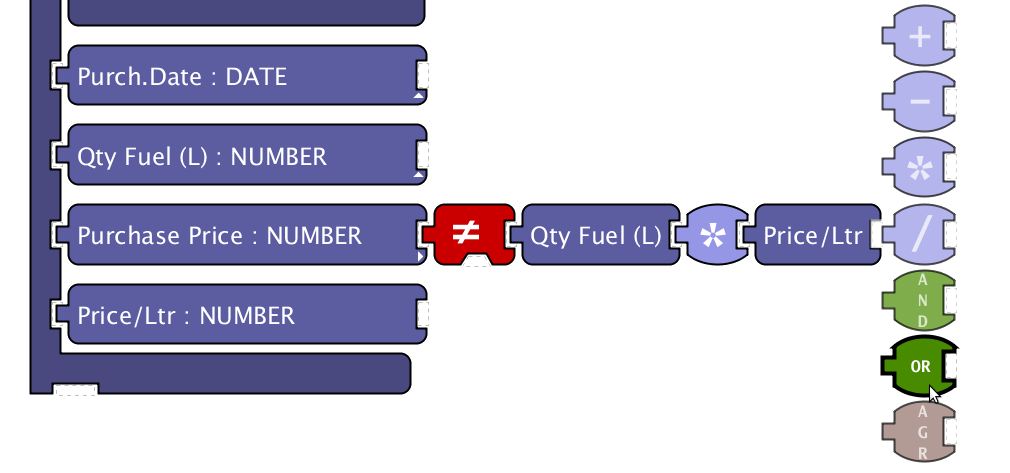
\includegraphics[scale=0.20]{images/01-rulesarea-suggestionmenu.png}  
		\vspace{-30pt} 
  	\end{figure}

	\BgThispage
\subsection*{Responsive HTML5 clients}
	TG employs an internal domain specific language for defining responsive Web UI.
	The UI concepts are all based on the business domain modelling principles to reinforce the world model metaphor, and follow the Google Material Design spec to deliver responsive and consistent User Experience (UX) across devices of multiple form factors.
	The TG presentation layer is based on Web Components (built with Google Polymer), which enables reuse and integration of in-house and $3^{rd}$ party components.
	TG offers a search-first approach to UX design that provides users with sophisticated first-class data retrieval tools supporting model-driven selection criteria, value autocompletion, ranges, meta-conditions (e.g. missing value, this year, previous fortnight), aggregations and sorting of the result sets. 

	
\subsection*{A software construction tool to facilitate the process management}
	Agile, Kanban, Scrum, FDD, TDD\ldots all of these and more are the management techniques, methodologies and methods to ensure the development of high quality and timely delivered software systems.
	These project management approaches exist for a good reason and there are multiple tools that assist with their implementation and practicing.
	This, however, is only one side of the coin.
	Implementing a proper process management method does not solve the software construction problem.
	It does not take away the technical needs and issues that arise during software construction.
	It can only help in mitigating them.
	That's why having an appropriate software construction tool that works well together with the process management method is vital to the success of any software project.
	Using the TG platform elevates software developers to the business domain level, establishes a ubiquitous business domain specific language to facilitate communication between the project stakeholders.


\subsection*{Robust Security}
	Industrial grade security, which includes HTTPS communication, the use of a key stretching PBKDF2 based password hashing, mutating session authenticator strategy, reduced sign-on with the support of both trusted and untrusted devices. 
	Support for multi-factor authentication scheme. 
	Declarative authorisation with pluggable backends (e.g. LDAP).

    
    
\subsection*{Cloud ready}
	Software systems built with TG are cloud ready.
	The platform employs RESTful architecture to structure application web-resources.
	This ensures clean separation between different business domain boundaries, UI resources and provides excellent capacity for scalability.

\subsection*{Complete application development lifecycle}
	One of the key meta-features of the Trident Genesis platform is its ability to support a complete lifecycle for developing software systems.
	This was one of our essential goals.
	Otherwise, there would always be low level technical aspects to software development that interrupt high level business domain oriented developer thinking.
	Thus, the development of software systems with TG covers all that is required for end-to-end software construction.
	This includes orthogonal aspects such as unit and functional testing, build and installation, business model design and database integration, UI definitions, secure HTTP communication, scalability and more.

\fi

%
% ---- Bibliography ----
%
\begin{thebibliography}{5}

\bibitem{Kay2003}
Kay, A. On the Meaning of ``Object-Oriented Programming''
\href{http://www.purl.org/stefan_ram/pub/doc_kay_oop_en}{Online}

\bibitem{Barnes:2007:ORM}
Bar\-nes, J.~M. Object-Relational Mapping as a Persistence Mechanism for Object-Oriented Applications, 2007,
\href{http://digitalcommons.macalester.edu/mathcs_honors/6/}{Online}

\bibitem{DeMichiel:2012:JPA}
De\-Mi\-chiel. L. JSR 338: Java Persistence API, Version 2.1, 2012,
\href{http://jcp.org/aboutJava/communityprocess/pr/jsr338/index.html}{Online}

\bibitem{evans2003}
Evans, E. Domain-Driven Design: Tackling Complexity in the Heart of Software, 2003, Addison-Wesley Professional.

\bibitem{Fowler:2010:DSL}
Fow\-ler, M. Domain-Specific Languages, Addison-Wesley Professional, 2010.

\bibitem{Fowler:2012:OH}
Fow\-ler. M. OrmHate, 2012,
\href{http://martinfowler.com/bliki/OrmHate.html}{Online}

\bibitem{Fielding2000}
Fielding, R. T. Architectural styles and the design of network-based software architectures: Phd thesis, University of California, Irvine, USA, 2000.

\bibitem{HBBPB:2008}
Hambrick, G. et al. Persistence in the Enterprise: A Guide to Persistence Technologies, 2008, IBM Press.

\bibitem{haywood2009}
Haywood, D. Domain-Driven Design Using Naked Objects, 2009, Pragmatic Bookshelf.

\bibitem{Hodych:2012}
Hodych, O. et al. Visual Domain-Specific Query Language for Business Applications, in Proceedings of 14-th International Conference on System Analysis and Information Technologies (SAIT 2012), Kyiv, Ukraine, 2012, pp. 311-312.

\bibitem{Hodych:2013}
Hodych, O. et al. Object-relational mapping: Limitations of data querying, in Proceedings of 15-th International Conference on System Analysis and Information Technologies (SAIT 2013), Kyiv, Ukraine, May 27-31, 2013. — P. 376–377.

\bibitem{HHN1986}
Hutchins, E., Holland, J. and Norman, D. Direct Manipulation Interfaces, in User Centered System Design: New Perspectives on Human-computer Interaction, 1986, CRC Press.

\bibitem{jacobson1992}
Jacobson, I. Object Oriented Software Engineering: A Use Case Driven Approach, 1992, Addison-Wesley Professional.

\bibitem{kal1983}
Kalinichenko, L. A. Methods and tools for integrating heterogeneous databases, 1983, Nauka (in Russian).
\foreignlanguage{russian}{Original title: Калиниченко Л. А. Методы и средства интеграции неоднородных баз данных, 1983, Наука.}

\bibitem{UBob:2002}
Martin, R.~C. Agile Software Development, Principles, Patterns, and Practices, 2002, Prentice Hall.

\bibitem{Neward:2006:VCS}
New\-ard. T. The Vietnam of Computer Science, 2006,
\href{http://blogs.tedneward.com/2006/06/26/The+Vietnam+Of+Computer+Science.aspx}{Online}

\bibitem{oli2007}
Oliv\'{e}, A. Conceptual Modeling of Information Systems, 2007, Springer.

\bibitem{pawson2001}
Pawson, R. and Matthews, R. Naked objects: a technique for designing more expressive systems, SIGPLAN Notices, V.36(12), pp.61--67, 2001.

\bibitem{pawson2004}
Pawson, R., Naked Objects, Ph.D Thesis, 2004, Trinity College, Dublin, Ireland.

\bibitem{vernon2013}
Vernon, V. Implementing Domain-Driven Design, 2013, Addison-Wesley Professional.

\bibitem{shneiderman1982}
Shneiderman, B. The future of interactive systems and the emergence of direct manipulation. Behaviour and Information Technology, 1(3):237–256, 1982.

\bibitem{shneiderman1983}
Shneiderman, B. Direct manipulation: A step beyond programming languages. Computer, 16(8):57–69, 1983.

\bibitem{fowler2003} Fowler, M. AnemicDomainModel, 
\href{http://www.martinfowler.com/bliki/AnemicDomainModel.html}{Online}

\bibitem{fowler2006} Fowler, M. DslBoundary, 
\href{http://martinfowler.com/bliki/DslBoundary.html}{Online}

\bibitem{bozhanov2010} Bozhanov, B. On Domain-Driven Design, Anemic Domain Model, Code Generation, Dependency Injection and More…
\href{http://techblog.bozho.net/on-domain-driven-design-anemic-domain-models-code-generation-dependency-injection-and-more/}{Online}

\bibitem{sapm2014}  The Anaemic Domain Model is no Anti-Pattern, it’s a SOLID design, The School of Informatics, University of Edinburgh,
\href{https://blog.inf.ed.ac.uk/sapm/2014/02/04/the-anaemic-domain-model-is-no-anti-pattern-its-a-solid-design/}{Online}

\bibitem{yegge2006} Yegge, S. Execution in the Kingdom of Nouns,  
\href{http://steve-yegge.blogspot.com.au/2006/03/execution-in-kingdom-of-nouns.html}{Online}

\bibitem{SOLID} SOLID (object-oriented design), 
\href{https://en.wikipedia.org/wiki/SOLID_(object-oriented_design)}{Online}

\bibitem{CQRS} CQRS design pattern, 
\href{https://cqrs.files.wordpress.com/2010/11/cqrs_documents.pdf}{Online}

\end{thebibliography}
%

\end{document}

